\chapter{Termo de Abertura do projeto}

\section{EAP}
\begin{figure}[!htb]
    \center{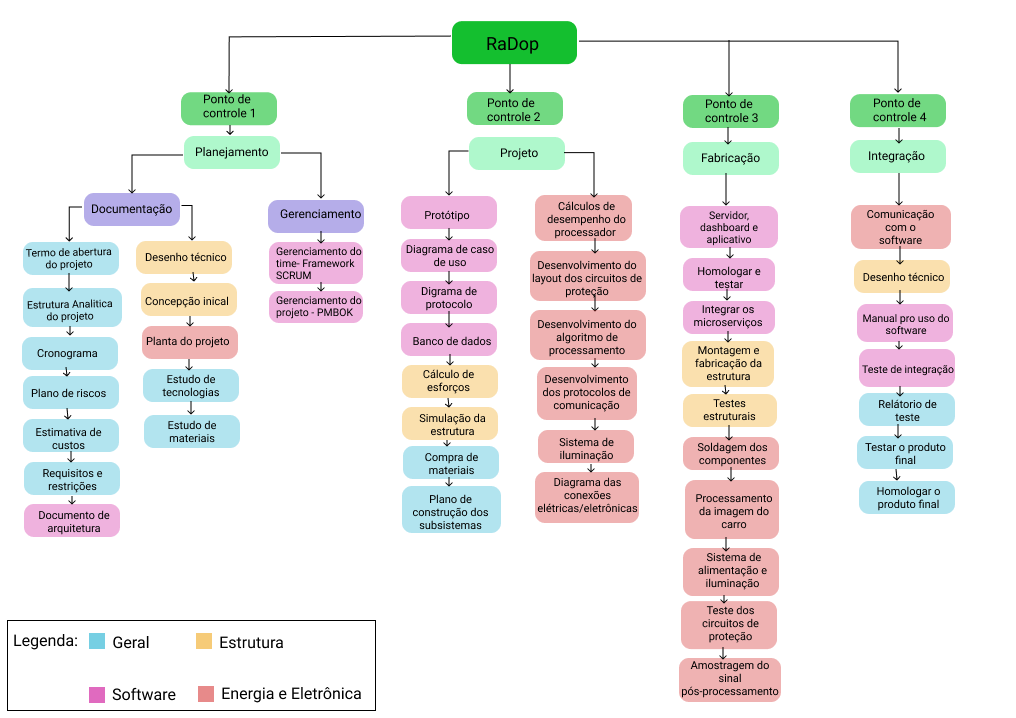
\includegraphics[width=\textwidth]{eap.eps}}
    \caption{\label{fig:eap} EAP do projeto}
\end{figure}
\section{Lista É/Não é}
\subsection{É}
\subsection{Não é}
\section{Requisitos}
\subsection{Eletrônica}
\subsection{Energia}
\subsection{Estrutura}
\subsection{Software}
\section{\emph{Stakeholders}}
\section{Recurso humanos}
\section{Cronograma de atividades}
\section{Milestones Identificados}
\section{Estimativa de custos}

\subsection{Engenharia de Software}

Aqui está listado todos os gastos que serão necessários para a equipe de software, assim como todas as aquisições que serão feitas durante o projeto:

\begin{table}[]
    \resizebox{\textwidth}{!}{\begin{tabular}{@{}|c|c|c|c|c|c|c|@{}}
    \toprule
    \textbf{Nome do produto} & \textbf{Descrição}                      & \textbf{Marca} & \textbf{Preço unitário} & \textbf{Quantidade} & \textbf{Fornecedor} & \textbf{Orçamento} \\ \midrule
    Servidor                 & Máquina para execução dos serviços      & ---            & US\$ 10,00 por mês      & 5 meses             & Digital Ocean       & US\$ 50,00         \\ \midrule
    Raspberry Pi 3 B         & Placa de IoT para execução de softwares & Raspberry      & R\$ 279,90              & 1 unidade           & FilipeFlop          & R\$ 279,90         \\ \bottomrule
    \end{tabular}}
\end{table}

OBS: Essa planilha poderá ser atualizado dependendo de necessidades que surgirem durante a execução do projeto.

\section{Viabilidades financeira}
\section{Levantamento de riscos}
